%!TEX root = ../thesis.tex

\chapter{Experimentelle Evaluation}
\label{chap:evaluation}
\todo{Evaluation füllen}
In diesem Kapitel wird nun analysiert wie zuverlässig und praktisch anwendbar die Implementierung ist. Zum einen wird die Performanz, der Implementierung betrachtet.  Zum Anderen wird die Qualität der Felderkennung betrachtet. 

Dabei wurden die Tests auf einem System mit Ubuntu 16.04 LTS und OpenCV Version 3.1 für Python 3 durchgeführt. Die hierbei genutzte Hardware ist ein Intel i7 4790k, mit 4 GHz und vier physischen Kernen. Zudem wurde eine Nvidia GTX 970 mit CUDA Support genutzt.
Die eingesetzte Kamera ist eine Logitech C310. Dieser verfügt über eine HD Auflösung mit  $1.280\times720$ bei $30FPS$. 

\begin{figure}[ht]
\centering
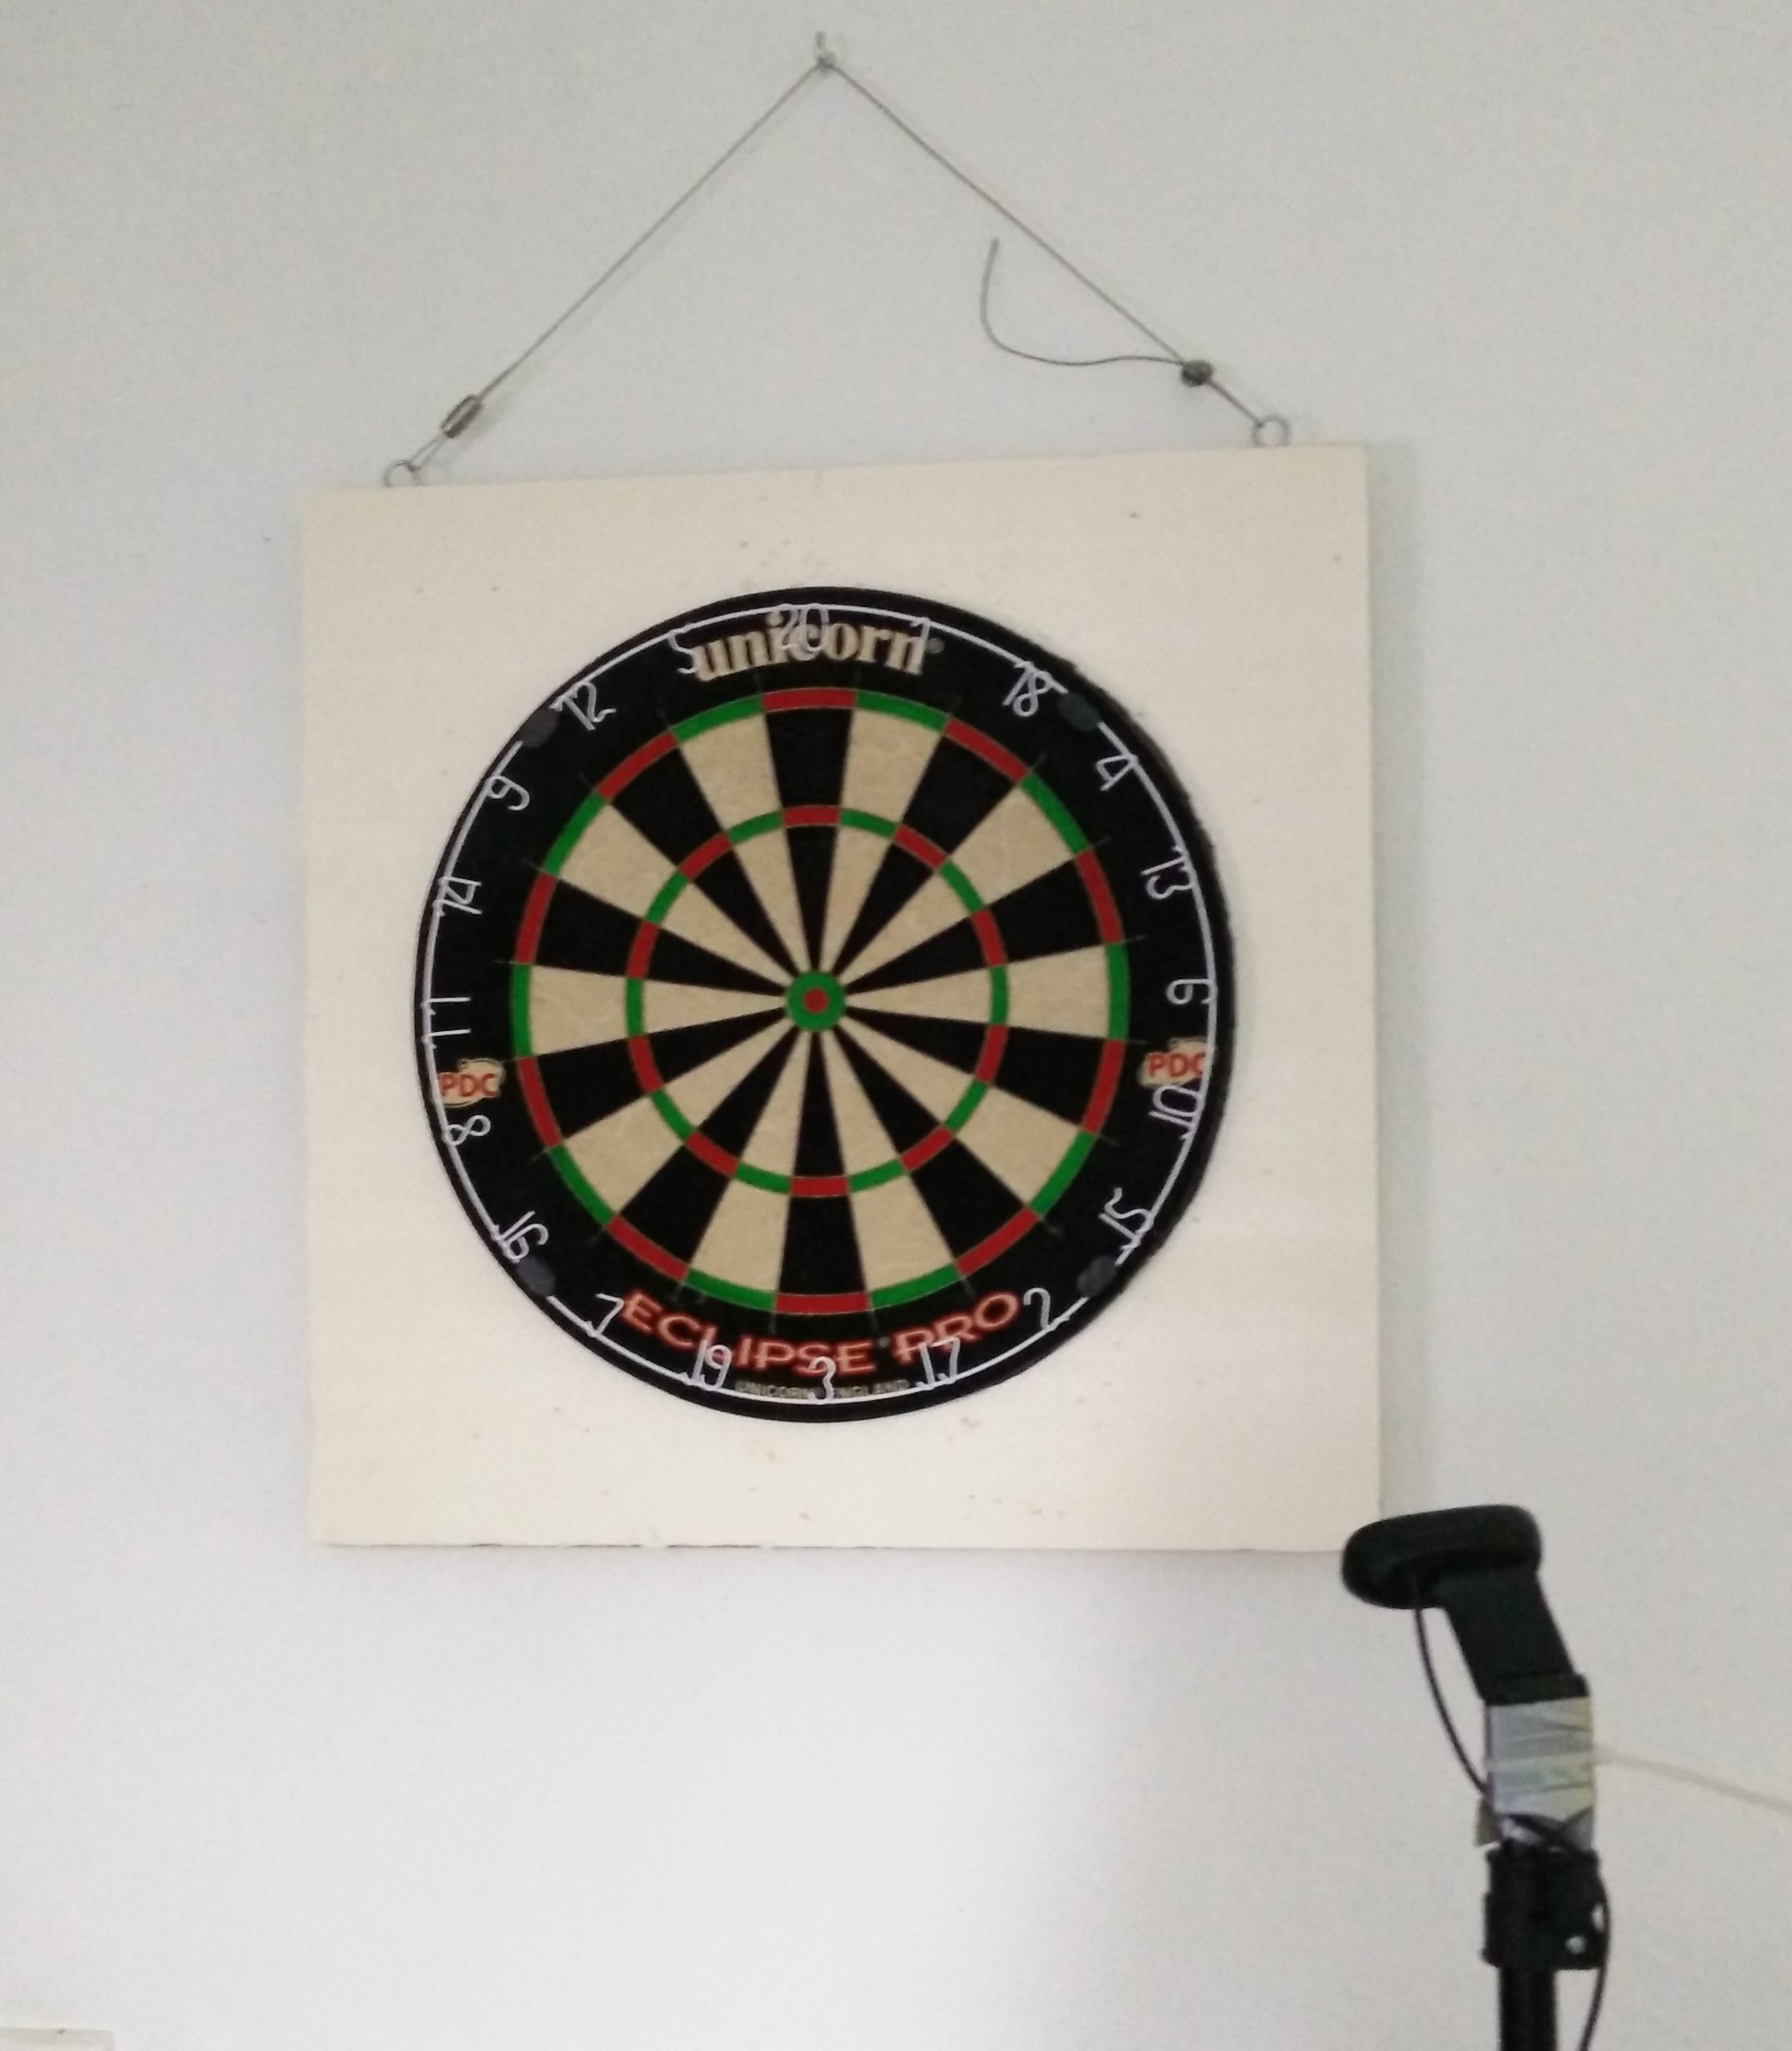
\includegraphics[width=0.6\textwidth]{media/testsetup}\\
\caption{\textbf{Zur Evaluation genutztes Setup}}
\label{Fig:testsetup}
\end{figure}
Dabei wurde die Kamera so aufgestellt, dass sie von unten seitlich auf das Dartboard gerichtet ist. In Abbildung \prettyref{Fig:testsetup} ist das Setup abgebildet. Damit wird verhindert, dass die Kamera sich in der Wurfbahn befindet. Es wurden konstante Lichtverhältnisse geschaffen, indem mit zwei Studioleuchten eine gleichmäßige Ausleuchtung geschaffen wurde.
\begin{figure}[ht]
\centering
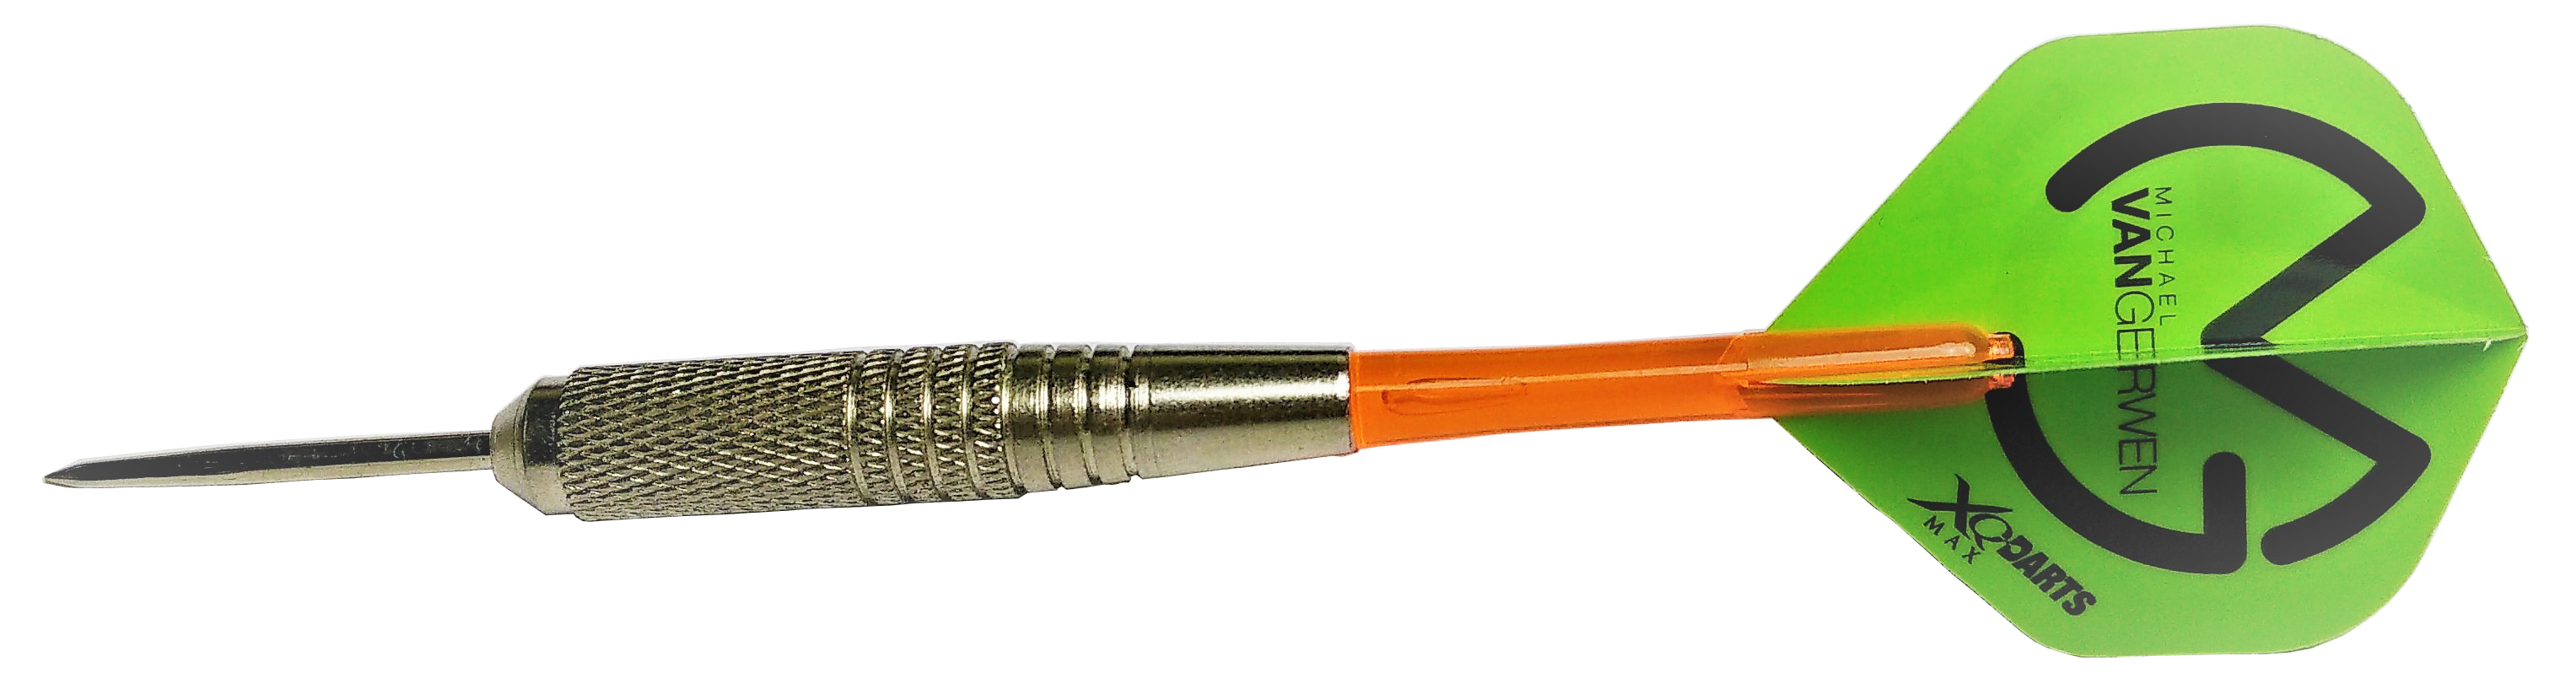
\includegraphics[width=\textwidth]{media/MyDart.png}\\
\caption{\textbf{Zur Evaluation genutzte Darts}}
\label{Fig:mydart}
\end{figure}

Zur Erfassung wurden X \todo{Anzahl der Testdaten eintragen} Testwürfe durchgeführt und aufgezeichnet. Damit eine möglichst große Streuung der Würfe gegeben ist, wurde nicht im klassischen Turniermodus vorgegangen. Stattdessen wurde, der im Kapitel \prettyref{sec:motivation} genannte, Modus "`Rennen"' genutzt, da es bei diesem das Ziel ist, jedes Feld auf dem Dartboard zu treffen. Würden die Würfe im Turniermodus gesammelt, so hätten sich die Würfe zu sehr auf eine Region konzentriert.
\section{Ergebnisse}
\label{sec:results}


\section{Grenzen der Analysemöglichkeiten}

